\section{LSTM Parsing Model}

\begin{figure*}[t]
\setlength\belowcaptionskip{-1em}
\centering
\captionsetup{justification=centering}
  \begin{center}
    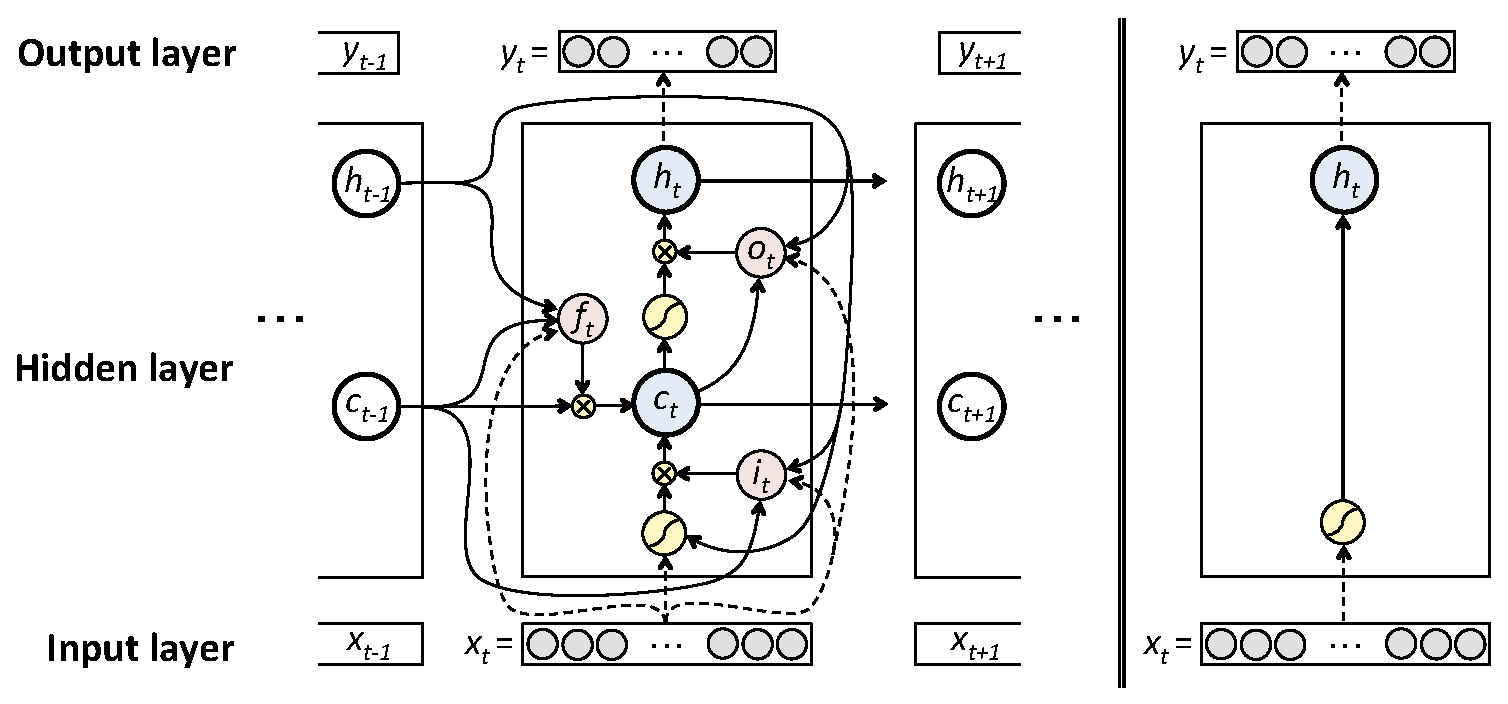
\includegraphics[width=0.85\linewidth]{images/fig_model.eps}
  \end{center}
  \setlength\abovecaptionskip{-.7truemm}
  \caption{Left: Our LSTM architecture. Right: Feedforward architecture in \newcite{chenmanning14}. Connections with dropout are denoted by dashed lines.}
\label{fig:model}
\end{figure*}

\subsection{Baseline Model}
Our model is an extension to \newcite{chenmanning14},
which uses a feedforward neural network to predict the next transition of an arc-standard system.
%In the arc-standard system, a configuration consists of a buffer $B$, a stack $S$, and a set of dependency arcs $A$.
%$B$ stores the input words, and the words are extracted from $B$ and pushed to $S$ as the dependency parsing proceeds and arcs are added to $A$.
In arc-standard, a configuration consists of a buffer $B$ (holding the input words), a stack $S$ (holding the partial parse trees), and a set of dependency arcs $A$.
The parse tree is built by successively making one of these transitions: 
\vspace{-.5em}
\begin{itemize}
\item SHIFT: move the next word on $B$ to $S$
\vspace{-.4em}
\item LEFT/RIGHT-ARC($L$): add left/right arc with label $L$ between top two words on $S$%, remove child
\end{itemize}
\vspace{-.5em}

%While feature engineering approaches like (Yamada and Matsumoto, 2003; Zhang and Nivre, 2011) use a classifier with sparse feature sets to decide which transition to take, the Chen and Manning model uses a feedforward neural network classifier with word, POS, and label embeddings as input features. In particular, their low-dimensional dense embedding features, which we term $x_t$, is a concatenation of embeddings from the top 3 words in $S$ and $B$, first and second left-/right-most children of the top two words on $S$, and the leftmost of leftmost / rightmost of rightmost children of the top two words on $S$. At each configuration at time $t$, the feedforward neural network first computes the hidden layer $h_t$ from the input $x_t$, then calculates the probability of each transition in the output vector $y_t:$\footnote{The dimension of $x_t$ is 2400 in experiments, and dimension of $y_t$ is $2|L|+1$, the number of possible transitions, with $|L|$ being number of dependency label types.}
The features $x_t$ is a concatenation of embeddings from the top 3 words in $S$ and $B$, first and second left-/right-most children of the top two words on $S$, and the leftmost of leftmost / rightmost of rightmost children of the top two words on $S$. At each configuration at time $t$, the neural network first computes the hidden layer $h_t$ from the input $x_t$ (applying a non-linear function $f$), then calculates the probability of each transition in the output vector $y_t:$\footnote{The dimension of $x_t$ is 2400 in experiments, and dimension of $y_t$ is $2|L|+1$, the number of possible transitions where $|L|$ = number of dependency label types.} %We omit bias terms in the equations for brevity.
\vspace{-1.0em}
\begin{eqnarray*}
  h_{t}\!\!\! &=& \!\!\! f (W_{xh} D(x_{t})) \\[-.2em]
  y_{t}\!\!\! &=& \!\!\! \mathrm{softmax} (W_{hy} D(h_{t}))
\end{eqnarray*}
$D(\cdot)$ is a dropout operator, which randomly sets elements to 0 with probability $p_{drop}$.
%$D(\cdot)$ is a dropout operator, which randomly sets elements to 0 with probability $p_{drop}$. In our notation, $W$ are matrix parameters to be learned and subscript like $W_{xh}$ indicate it connects $x$ (input) to $h$ (hidden layer). We ignore bias terms in the equations for brevity, though they are used in practice. 

\vspace{-.5em}
\subsection{Our LSTM Model}
%Our LSTM model uses the same $x_t$ features as (Chen and Manning, 2014), but importantly adds new inputs based on past information, e.g. previous hidden layer $h_{t-1}$. The addition of previous state leads to recurrence and thus theoretically enables modelling and training of the entire sequence of transitions. 
Our LSTM model (shown in Figure~\ref{fig:model}) uses the same $x_t$ features as \newcite{chenmanning14}, but importantly adds new inputs based on past information (such as $h_{t-1}$). The addition of previous state leads to recurrence and enables modelling and training of the entire sequence of transitions. 
%In practice, recurrence may cause the infamous "exploding gradient" and "vanishing gradient" (Bengio et al., 1994) problems, which lead to numerical difficulties in backpropagation training. 
%LSTM units provide an effective way to circumvent these numerical problems by introducing memory cells $c_t$ that could store information over long time intervals. What is stored in a memory cell $c_t$ is controlled by an input gate $i_t$, and whether the stored information is used in further computations is controlled by an output gate $o_t$. This allows information from the beginning of the sentence to influence transition actions at the end of the sentence. A forget gate $f_t$ is used to erase the information in the current memory cell. 

While recurrence may cause the ``vanishing gradient'' problem \cite{Bet94},
the LSTM architecture solves this by introducing memory cells $c_t$ that could store information over long time intervals and keep gradients from diminishing. Input gates $i_t$ control what is stored in a memory cell $c_t$, and output gates $o_t$ control whether the stored information is used in further computations. This allows information from the beginning of the sentence to influence transition actions at the end of the sentence. Forget gates $f_t$ are used to erase the information in the current memory cell. 

%The following equations describe our LSTM parser with peephole connections (Gers et al., 2002). Figure~\ref{fig:model} shows how each of the components connects. This LSTM unit setup follows the strategy set forth by~(Graves, 2013), while the recipe for successfully applying dropout to LSTM was investigated in Zaremba et al. (2014).
The following equations describe our LSTM model with peephole connections \cite{Get02}, as set forth by \newcite{G13}, and apply dropout similar to \newcite{Zet14}.
\vspace{-.6em}
\begin{eqnarray*}
  i_{t}\!\!\! &=& \!\!\! \sigma (W_{xi} D(x_{t}) + W_{ci} c_{t-1} + W_{hi} h_{t-1}) \\[-.25em]
  f_{t}\!\!\! &=& \!\!\! \sigma (W_{xf} D(x_{t}) + W_{cf} c_{t-1} + W_{hf} h_{t-1}) \\[-.25em]
  c_{t}\!\!\! &=& \!\!\! f_{t} c_{t-1}\! + \!i_{t} \ tanh (W_{xc} D(x_{t})\! + \!W_{hc} h_{t-1}\!) \\[-.25em]
  o_{t}\!\!\! &=& \!\!\! \sigma (W_{xo} D(x_{t}) + W_{co} c_{t} + W_{ho} h_{t-1}) \\[-.25em]
  h_{t}\!\!\! &=& \!\!\! o_{t} \ \tanh(c_{t}) \\[-.25em]
  y_{t}\!\!\! &=& \!\!\! \mathrm{softmax}(W_{hy} D(h_{t}))
\end{eqnarray*}

\vspace{-.6em}
%Crucially, the difference between the LSTM parser and feedforward parser is that the LSTM not only uses input $x_t$ in its predictions for $y_t$, but also exploits values in the previous memory cell $c_{t-1}$ and hidden layer $h_{t-1}$. Note that the gates $i_t$, $f_t$, and $o_t$ are bounded between $[0,1]$ due to the sigmoid $\sigma$, so their multiplication with other parts of the network modulates which information is passed through, e.g. $f_t$ and $i_t$ determine how much of the current memory $c_t$ depends on previous memory $c_{t-1}$, or current input $x_t$ plus previous hidden layer $h_{t-1}$. The gates have their own parameters (e.g. $W_{xi}$) and are learned jointly via backpropagation. 
Crucially, the LSTM not only uses input $x_t$ in its predictions for $y_t$, but also exploits values in the previous memory cell $c_{t-1}$ and hidden layer $h_{t-1}$ through the gates $i_t$, $f_t$, and $o_t$. The values of these gates are bounded between $[0,1]$ due to the sigmoid  $\sigma$, so multiplication with other components modulates what information is passed through. 

Given training sentences ${\{s_{i}\}}_{i=1}^{m}$ with gold parse trees,
our training data is a set of sequences of configurations $c_{it}$ and oracle transition actions $a_{it}$ at each time $t$ for each sentence $s_{i}$.
We maximise the log-likelihood of the oracle transition actions $a_{it}$ given by Equation (\ref{eq:ll}),
where $\theta$ is the set of parameters including word, POS, and label embeddings,
and $y_{t}(a)$ is the probability that the parser takes transition action $a$ at time $t$.
\vspace{-1em}
\begin{equation}
  L(\theta) = \sum_{i=1}^{m} \sum_{t} \log y_{t}(a_{it})
  - \frac{\lambda}{2} ||\theta||^2
  \label{eq:ll}
\end{equation}

\vspace{-1em}
We optimise by gradient backpropagation through time (BPTT) for each sentence $s_{i}$, feeding the parser with gold sequence of configurations $\{c_{it}\}_{t=1}^{|s_{i}|}$. 
When the parser reaches the final configuration, the gradients are backpropagated
from each prediction ${y_{it}}$ at time $t$ down to time $1$.